
Emocionados antes de la salida a nuestro segundo viaje en bici, y luego de armar
el equipaje y comprobar que quedara firmemente sujeto al portapaquetes, un d\'ia
antes de la partida salimos, a la hora de la siesta, a dar una vuelta con bicis
cargadas por Pergamino. Euf\'oricos por el inminente proyecto recorrimos el
centro, anduvimos a distintas velocidades, comprobamos si las alforjas
molestaban al pedaleo, y cruzamos a pocos amigos, de quienes nos despedimos.

Volviendo a casa nos sorprendi\'o un diluvio de verano que nos empap\'o tanto
como a nuestro equipaje, y as\'i probamos que las nuevas alforjas \emph{no son}
impermeables: hay que cubrirlas bajo la lluvia. Mejor tarde que\ldots\
\textexclamdown demasiado tarde!

La siguiente ma\~nana subimos al colectivo con nuestro equipaje sucio y mojado,
\textexclamdown como si estuvi\'eramos llegando en lugar de empezando!

\section{San Rafael y el Ca\~n\'on del Atuel}

\subsection*{Lunes 3 de Enero de 2005}

El colectivo ``{\small TAC}'' que nos llevar\'ia hasta la terminal de San Rafael
quem\'o su embrague 30~km antes del destino, as\'i que, con la ansiedad que ya
nos movilizaba, tomamos nuestro equipaje, quitamos los cartones de las bicis,
las armamos y empezamos a pedalear. Los pasajeros y el conductor nos miraban
sorprendidos, este \'ultimo nos dej\'o varias galletitas que usan en los
desayunos para nuestra jornada. Malo el coche, pero esa ansiedad no nos
permiti\'o verlo. Nos calm\'o salir antes, pero no fue la mejor idea porque nos
separaban a\'un 50~km del primer paisaje bonito: el Ca\~n\'on. Antes, planicie
\'arida con muchos \'alamos. {\small TAC} arregl\'o su veh\'iculo, y al pasarnos
nos tocaban bocina y hac\'ian se\~nas de luces: ``\textexclamdown buen viaje!''

Nada muy interesante por estos kil\'ometros, solo el hecho de estar sobre
nuestras bicis en suelo mendocino (nuevo para nosotros), con alforjas y
respectivas banderitas argentinas. Entramos en una bodega que cruzamos,
interesante conocer pero nada que me atrape.

A los 50~km empez\'o el ca\~n\'on, donde pinchamos una rueda que se repar\'o
r\'apidamente. Cambiar la c\'amara delantera es m\'as f\'acil porque no lleva el
peso. Pasamos a un grupo de treinta ciclistas adultos reunidos en la banquina,
que ten\'ian colectivo de apoyo. Nos saludaban muy cari\~nosos gritando:
\emph{``\textexclamdown \'eeesos son ciclistas!''} Es important\'isimo el apoyo
y afecto de la gente para mantenernos incentivados y con toda la energ\'ia para
el viaje. Devolvimos agradecidos sus saludos sin dejar de pedalear.

Recorrimos luego 25~km de este paisaje lindo, es decir, completamos 75~km en el
primer d\'ia. A orillas del r\'io Atuel, en un lugar barato y lindo armamos
campamento. Por ese r\'io pasan m\'as raftings que colectivos por una avenida
porte\~na, y es tan calmo que decidimos que si subimos a un bote lo haremos
en Uspallata por el r\'io Mendoza, m\'as movido. Se ver\'a.

Cena, y a descansar.

\subsection*{Martes 4 de Enero}

Descansamos bien pero, quemados por el sol, decidimos esa ma\~nana postergar la
salida. Hab\'ia un sol radiante, as\'i que nos metimos en el r\'io y caminamos
un poco por el lugar. Pasamos las horas de la siesta bajo la sombra de un buen
\'arbol, echados sobre las bicis cargadas.

Todav\'ia frescos por el chapuz\'on salimos a pedalear; imponente el Ca\~n\'on
del Atuel. Despu\'es de una sinuosa subida y t\'unel cruzamos el primer dique: a
su derecha se muestra el gran lago que forma, y a su izquierda, un peque\~no y
lejano cursito de agua. Durante la subida ve\'iamos la inmensa pared de
hormig\'on acercarse, impresiona. No estaba trabajando en ese momento.

La subida era larga y en curvas, el paisaje mutaba constantemente. El cielo
atr\'as estaba claro como en una playa veraniega, y adelante estaba azul oscuro
y de grises, parec\'ia una gran tormenta. \textexclamdown Nos inquietaba que
lloviera! Para proteger el equipaje lo cubrimos con nylon, poco est\'etico pero
\'util. Par\'abamos en cada curva que hubiera guarda riel donde apoyar las bicis
para mirar al paisaje, comer las barritas de cereales que nos regalaron en
Navidad, y para descansar de la subida que nunca terminaba. Y seguimos subiendo
intensamente hasta llegar a la cima del cerro. Pero ah\'i no era la cima,
aparec\'ian curvas y ondulaciones, y las seguimos subiendo, hasta el punto m\'as
alto. \textquestiondown Pero los cerros crecen ac\'a? Subimos un poco m\'as (se
hizo \emph{largo}) para llegar a la cima de verdad, desde donde pod\'iamos ver
con ojitos asombrados la bajada que nos esperaba.

\textexclamdown Por fin el placer! Y para aumentarlo empezaba una fina
lluviecita, las curvas de ripio exigir\'ian m\'as atenci\'on. Nos sacamos fotos
arriba (las caras de loco suelto dan gracia) y comenzamos. Unas piedrotas
--imposibles de ver por la lluvia que ba\~naba la cara-- sobresal\'ian del
camino. \textexclamdown Cuando me sorprendi\'o la primera casi pierdo el
manubrio y beso al piso! Pero por suerte no pas\'o, y segu\'i acelerando
agarrado m\'as firmemente para poder pasar por sobre las otras cada vez m\'as
r\'apido, r\'igido sobre la bici, sin sentarme por supuesto. Inolvidable, la
suspensi\'on gritaba un sonido met\'alico en cada choque, salvaba mis mu\~necas
y equilibrio. \textexclamdown Y c\'omo se sent\'ia estar ah\'i arriba! Sumado a
la velocidad, la tierrita ba\~nando la cara y bici, las alforjas
balance\'andose, el olor a tierra mojada, estar en Mendoza\ldots\ Alegr\'ia.

A 25~km del primer campamento llegamos a un lugar sin pendiente donde paramos a
tomar agua, miramos hacia abajo, y encontramos un valle con \'arboles y plantas
verdes. Incre\'ible, s\'olo se ven arbustos bajos por esta zona, pero \'este
parec\'ia un rinconcito de Villa la Angostura. El r\'io cerca, y una islita de
piedras en el medio sonar\'ian toda la noche. Eso es lo lindo de viajar a pedal:
es m\'as f\'acil de llegar a ver esos rincones. Quer\'iamos bajar, pero hab\'ia
una cuesta empinada de piedras sueltas, imposible con todo cargado. Pedaleamos
hasta encontrar un buen lugar por donde acercarnos; cruzamos por ah\'i un cartel
anunciando la prohibici\'on de acampar: ``el uso de diques puede inundar la
zona''. Por eso ser\'ia tan f\'ertil esa tierra.

Llegamos a una bajada menos intensa y, uno arriba y el otro abajo, nos
arreglamos para mover las bicis, cargadas como mulas. Echamos la carpa en unas
hierbas altas que hac\'ian de colch\'on (impensable en un viaje de mochilero, y
menos por zonas \'aridas), al lado de un \'arbol de esos viejos y muy grandes,
donde cocinar\'iamos los capeletinis. Hicimos un tesito a orillas del
r\'io\ldots\ lo \'unico que molestaba eran unas mosquitas que ni siquiera
picaban (recordando los t\'abanos del sur, invalorable). Para\'iso.

``Hacer un tesito'' de viaje significa bajar al r\'io a buscar agua fresca,
traerla en un tarro de lata, encender un fuego con ramas y alg\'un tronquito, y
(si no se pudo de modo m\'as simple, como esta vez) sostener durante 5 minutos
con una rama gruesa y verde la lata sobre el fuego. Las tacitas son de
pl\'astico: tomar de un recipiente de lata quemar\'a irremediablemente los
labios. \textexclamdown Ese es el ``placer'' del t\'e de mochilero!

\begin{center}
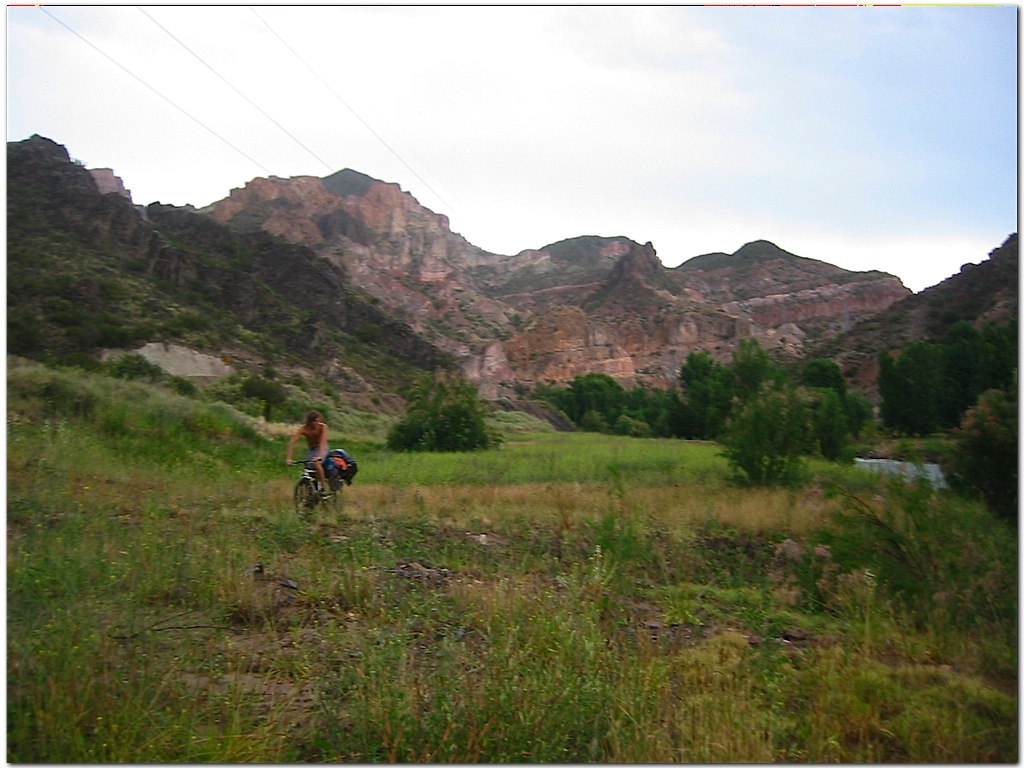
\includegraphics[width=300px]{images/Mendoza_0196.jpg}\\
\textsc{Como en casa.}
\end{center}

Cruzamos a la islita del r\'io, pisando las piedras grandes para estar firmes.
La correntada era fuerte, pero al pasar m\'as baja que nuestra cintura nos
permit\'ia caminar. Yo cruc\'e primero, y, para no mojar dos pares de
zapatillas, ten\'ia que tirarle a Eze mi par. \textexclamdown Con errar un tiro
perd\'ia mis zapatillas en el r\'io y se terminaba el viaje! Pero un poco
nervioso y otro divertido llegu\'e a tirarlas, as\'i que bien calzado Eze
cruz\'o a la islita. \textexclamdown Agua \emph{fr\'ia}! Empezaba justo una
lluviecita fina con sol, ver las gotas iluminadas caer, refrescando, me hizo
sentir en un oasis. Miramos alrededor, dijimos ``esto es lo que queremos'', y
volvimos a buscar troncos para mantener un largo fuego despu\'es de la cena.

Mientras busc\'abamos los le\~nos empez\'o a sonar una tenebrosa y fuerte
sirena, \textexclamdown peor que las de los bomberos! Y qu\'e m\'as pod\'ia
ser que el cercano dique, si ah\'i hay \emph{nada}. Me desesper\'e. Volvimos a
fondo al campamento, lo primero que hice fue subir la bici hasta un lugar alto,
en la cuesta de las piedras sueltas. Estaba asustad\'isimo, porque imaginaba esa
imagen de dibujitos animados en que viene una ola enorme que se lleva todo, y
Eze, m\'as tranquilo, se descostillaba de la risa de s\'olo ver mi cara. Cuando
me tranquilic\'e un poco y entend\'i que no era as\'i de grave intent\'e bajar
la bici, pero no pod\'ia. La hab\'ia subido tanto como nunca hubiera podido:
\textexclamdown era imposible subirla hasta all\'a corriendo a trav\'es de las
piedras sueltas! Ahora no par\'abamos de reirnos.

``\textquestiondown Y ahora qu\'e hacemos?'' El campamento estaba armado.
\textexclamdown Toda esa noche estaba armada! Clavamos una rama a orillas del
r\'io para comprobar que el nivel empezaba a subir, y s\'i; nos exigi\'o
levantar campamento al hundirse lentamente. Todo lo que desarmamos,
\textexclamdown todo!, de nuevo sobre las bicis. Alrededor de las 9 de la noche,
cuando todav\'ia ni hab\'iamos cenado. Triste pero as\'i era la vida. Armamos
todo, y repet\'i la foto que sacamos al llegar mostrando al campamento, pero
ahora enfrente no hab\'ia m\'as que el paisaje y la carpa doblada sobre el
pasto. Por la poca luz y mi mal pulso (entre nervios y cansancio) sali\'o
movida. \textexclamdown Como para olvidar el momento!

Abandon\'abamos nuestro lugarcito saliendo por el barranco ``f\'acil''.
Volvimos unos metros por la ruta para sacarnos una foto con el amigable cartel
``prohibido acampar'' y, \textquestiondown qu\'e encontramos a su lado? Un
camino perfecto para subir y bajar pedaleando al mismo valle. En la emoci\'on lo
pasamos por alto y tuvimos que hacer malabares para transportar la carga.

Empezamos a andar de noche. Est\'abamos un poco cansados por el kilometraje del
primer d\'ia y la subida de hoy, pero no pod\'iamos hacer otra cosa. Salieron
todas las estrellas que pudieron pero la luna no se asom\'o, es la luna nueva
m\'as inoportuna que me haya tocado. Nos iluminaba una humilde linternita
encintada a mi manubrio, entre su poca iluminaci\'on y mi mareo a veces perd\'ia
la l\'inea del camino. \textexclamdown Y el compa\~nero que segu\'ia mi huella
me retaba por no ir por el medio! Poca agua y mucho cansancio para m\'i me
dejaron con baja presi\'on, me costaba enfocar. Cuando la rueda delantera
empezaba a saltar, o el pedal izquierdo a tocar la tierra acumulada en la
banquina, era se\~nal de no estar avanzando por donde quer\'iamos.
\textexclamdown Gracioso por el final feliz! (No nos ca\'imos al r\'io.) Pasamos
un restaurant y un dique, buscando otro cuadrado de pasto donde armar la carpa.
Por el camino, simplemente, no hab\'ia lugar.

Los diques son algo impresionante, sobre todo para estos dos estudiantes de
Ingenier\'ia. Es interesant\'isimo estar sobre esas moles que vibran tanto para
producir, de la fuerza del agua bajando, energ\'ia para las licuadoras y
bombitas de luz de las casas. Qu\'e ingenio.

Volviendo a nuestro problema, a medida que avanz\'abamos buscando un cuadrado
libre de arbustos y fuera del paso, el camino se tornaba m\'as angosto y
des\'ertico.

En el camino encontramos un t\'unel escarbado en la piedra de la monta\~na.
Oscuridad plena adentro, y las linternas con suerte llegaban a iluminar el
rugoso techo. No pod\'iamos saber el largo, ver si era en curvas, si habr\'ia
alguien adentro, si nos chocar\'ian\ldots\ Llev\'abamos una baliza en la parte
trasera de las alforjas para ser vistos. Pero, \textquestiondown y si ven\'ia
alguien medio dormido? Dejamos las bicis sobre el camino pensando todas estas
cosas y, seguramente, exager\'andolas. Por supuesto no nos quedar\'iamos hasta
que saliera el sol, as\'i que volvimos a montarlas y encaramos esos metros. Si
alguien nos tomaba del hombro o nos gritaba cerca, con plena seguridad se nos
deten\'ia el coraz\'on.

Y en plena oscuridad y con los ojos abiertos muy grandes, avanzando lentamente,
se escuch\'o un \emph{``\textexclamdown \textexclamdown ch\'annk!!''} Y\ldots\
\textexclamdown luz! Al hablar lo hac\'iamos murmurando, as\'i que mi alarido,
y su correspondiente eco, se hicieron notar. \textexclamdown Ahora no pod\'iamos
parar de reir! Habr\'ia sensores que al notar movimiento encender\'ian las
luces, igual nunca escuch\'e un encendido tan ruidoso. Aunque no tengo dudas de
que al venir asustado y dormido lo magnifiqu\'e. Cruzamos el t\'unel, no
recuerdo si por el tiempo que demoramos las luces se volvieron a apagar y a
prender, pero ya est\'abamos adentro y advertidos del ruido que provocar\'ian.

Pasada la medianoche y a\'un sin comer, nos sentamos sobre el camino para
descansar un rato. El cansancio molestaba. Comimos bastante chocolate
``Cabsha'', me dej\'o tan asqueado que a\'un me invade una fea sensaci\'on con
s\'olo ver el paquete. Imaginen empezar a andar en bicicleta ya cansados, con
est\'omago vac\'io, y, horas despu\'es, literalmente en medio de una noche y
del camino, esperando un lomo completo con huevo y muchos aderezos, abrir el
pl\'astico del chocolate medio derretido, y comerlo en abundancia.
\textexclamdown Disgust\'o! Pero ten\'ia hambre. Cuando hay hambre s\'i hay pan
duro, pero se lo come igual.

Era la una de la madrugada cuando llegamos al siguiente dique asesino de
acampantes, para cenar los tan esperados capeletinis. Ayer comimos polenta con
tuco, pero esta vez el plato no gozaba siquiera de un saborizante. El precavido
de mi compa\~nero llev\'o atados los le\~nos que \'ibamos a usar en la cocinita
de aquel valle, una salvaci\'on. Todav\'ia me pregunto c\'omo logr\'o
encenderlos: conseguir ramas en estos paisajes no es tarea f\'acil. Los comimos
sentados sobre el gran muro de ese dique, con las piernas colgando sobre la gran
ca\'ida, mirando al vac\'io y el agua caer. Algunos reflectores iluminaban la
obra, era en verdad espectacular.

Hasta el otro dique nos separaba poquito, 8~km creo. Claro que en ese momento
eran mortales para mi, pero no significaban una locura. \textexclamdown La
situaci\'on entera era una locura en realidad!

La suma tiene que dar 118~km para esta noche en que armamos la carpa en una
placita, al lado del dique cuarto. Me tir\'e as\'i nom\'as, con todas las
botellas vac\'ias alrededor, y palm\'e instant\'aneamente agradeciendo ese
pedazo de pasto. ``Prohibido acampar'' en ese parquecito de la entrada,
obviamente, pero de verdad ya no quedaba otra posibilidad. Eran las 3am al
momento de dormirnos. Un d\'ia que no podemos tildar de aburrido.

\subsection*{Mi\'ercoles 5 de Enero}

Alrededor de las diez de esa ma\~nana me despert\'o el calor del sol sobre la
carpa. La micci\'on amarilla intensa revelaba mi deshidrataci\'on. Dolor de
cabeza al moverme y esa cosquilla anterior al calambre constantemente presente
en las piernas confirmaban.

Se despert\'o Ezequiel, y entramos al dique a pedir agua. El gran ruido de las
turbinas nos imped\'ia anunciarnos a dos obreros que trabajaban del otro lado de
la entrada. Entr\'e en la cocina, hab\'ia un dispenser de agua, de los de
oficina. Entre lo que tom\'e en ese momento y las botellas que llen\'e, lo
vaciamos. Ezequiel se preocupaba un poco porque nadie sab\'ia que hab\'iamos
entrado, pero yo me sent\'ia mal, y no me incomodaba nuestro exceso de
confianza. Tom\'e hasta saciarme, y ya me sent\'ia mejor. Cansado f\'isicamente,
pero bien dormido.

Antes del mediod\'ia partimos hacia el Nih\"uil, donde dormir\'iamos aquella
noche. Entre 10 y 15~km no sonaban demasiado, pero unos caracoles en subida en
ripio me terminaron de fulminar. Color verde por el cansancio, me puse verde
claro cuando vi los caracoles desde arriba: \textexclamdown qu\'e bien luc\'ian!
Nuestros primeros caracoles, \textexclamdown y de subida! Las familias sub\'ian
y bajaban en auto, tomando mates y comiendo galletitas o facturas. A nosotros se
nos ca\'ian las babas como a perro. No se imaginan c\'omo empec\'e a valorar el
auto, las comidas, la limpieza\ldots\ y el Viaje.

Llegar a El Nih\"uil fue al principio una liberaci\'on, despu\'es una mala
sorpresa. \textexclamdown Era vac\'io el lugar! Una ciudad que comparo con
Urquiza, pueblo aleda\~no a Pergamino de poca belleza, pero con un dique feo, y
un lago con playas sin sombras donde descansar por detr\'as. Ser\'a que mi
cansancio no me permit\'ia disfrutar, porque diques los hay en todo el camino y
siempre me cautivaron. Pero de \'este, que era tan grande, recib\'ia una pared
de hormig\'on m\'as que un logro de la Ingenier\'ia. Es realmente importante
estar bien an\'imicamente, de eso depende no s\'olo llegar sino tambi\'en
disfrutar el viaje. No pod\'iamos perder tiempo durmiendo ah\'i, pero estaba
moribundo. \textexclamdown Para colmo, los campamentos cobraban como una
hoster\'ia barata en San Mart\'in de los Andes! Y alojaban a gente grande en
auto, no sent\'iamos afinidad.

Almorzamos muy bien, un s\'andwich de milanesa grande y completo, que para comer
tuvimos que salir del restaurantito para que no nos cobren el ``servicio''. No
recuerdo que estuvi\'eramos tan sucios pero es altamente probable. Dormimos una
reparadora siestita en una plaza, y decidimos que volver\'iamos en colectivo a
San Rafael por mi cansancio, pero cuando el chofer se levant\'o de su siesta, me
dijo que las bicis no entraban.

Averig\"uamos que el camino de vuelta era pavimentado, de 20~km hasta El
Desv\'io, un cruce de rutas con parador; y 20~km desde all\'i hasta la Cuesta de
los Terneros, donde empieza una bajada en curvas (de alrededor de 30~km) hasta
San Rafael. 70~km totales. Conclusi\'on: a pedalear para El Desv\'io, que estaba
a mitad de camino de la Cuesta de los Terneros. Ruta desierta, recta y plana;
\textexclamdown m\'as cansadora que los caracoles de ripio y en subida!

Al llegar tom\'e poca chocolatada porque estaba asqueado, y com\'i una
zanahoria; impensable al llegar a un lugarcito donde poder comprar dulces.
\textexclamdown No se asusten que durante el pedaleo, las barras de cereales y
el agua en botellas de 2 litros son moneda corriente! Nos contaron ah\'i que la
noche anterior hab\'ia granizado por la zona y en el dique ni nos enteramos,
\textexclamdown qu\'e buena suerte! Me qued\'e una hora sentado hasta
recuperarme un poco, viendo las chatitas tur\'isticas ir y venir. Era un lugar
de paso, aburrido; y si bien quer\'ia armar la carpa al costado preferimos
seguir hasta la Cuesta de los Terneros y ver menos turismo. Con un poco de
esfuerzo llegar\'iamos, como lo hicimos hasta El Desv\'io.

Pero esta vez era una larga recta en subida suave que no se llega a notar, y uno
avanza entonces frenado sin saber porqu\'e. El paisaje permit\'ia ver por
kil\'ometros la extensi\'on de ruta que faltaba. No hab\'ia carteles, y los
mojones no se acercaban por mucho que pedale\'aramos. En un cruce de caminos
hab\'ia una garita para colectivos, la mir\'e con cari\~no para pasar la noche,
pero ol\'ia muy mal y no nos dejaba c\'omodos.

Ahora estaba verde militar no oscuro, y Eze me habr\'a querido matar, pero justo
antes de la bajada caracoleada de los Terneros, anunciada por un bello cartel,
dije: ``\textexclamdown Basta! Paremos ac\'a porque muero sino''. A esos 20~km
del Desv\'io est\'abamos en la cima de todo el recorrido, el punto m\'as alto.
48~km en subidas este d\'ia en que me duraba a\'un el cansancio de ayer. Y
seguimos subiendo unas dos cuadras para llegar al monumento de San Francisco de
As\'is, donde ahora s\'i dormir\'iamos. Usamos unas 5 o 6 horas en completar
este recorrido. De ah\'i se ve\'ia todo divino, pero no lo pude apreciar mucho
esa tarde. Ezequiel s\'i, recorri\'o y sac\'o las fotos que yo no quise ni pude.

Arm\'e la carpa sin estacas ni sobretecho, sobre un suelo duro e irregular, y
dorm\'i una siesta de una hora en el anochecer. Es bueno dormir, repara r\'apido
la mala onda del cansancio f\'isico. El cansancio persiste pero la mala onda no.
Ezequiel termin\'o con el armado de carpa, y cenamos galletitas con pat\'e, para
no armar el fuego y por mi asqueo. Y ca\'i dormido r\'apidamente.

Antes de la medianoche empez\'o a soplar un ventarr\'on que tumbaba la carpa. Y
nos dimos cuenta: \textquestiondown c\'omo armar la carpa en la punta de un
cerro mendocino? El fuerte viento la mov\'ia golpeando mis pies, despu\'es de un
corto sue\~no me despert\'e sobresaltado. Todav\'ia nos re\'imos porque
empec\'e:

\subparagraph{}\label{ssub:tormenta}
--- \textexclamdown Zequi\'el, zequi\'el! \textexclamdown Se rompi\'o la carpa!
  Zequi\'el, \textexclamdown despertate!\\
\hangindent=1.6cm

Yo no entend\'ia nada, me costaba moverme, y el muchacho no respond\'ia. Al
tocarlo me pregunt\'o para qu\'e lo molestaba; le expliqu\'e, me reincorpor\'e y
segu\'i con la mano todo el per\'imetro que me rodeaba, \textexclamdown estaba
impecable! Algo golpeteaba y entredormido pens\'e que se hab\'ia roto una pared.
Si no era por las estacas despu\'es puestas, en ese momento se desarmaba todo.

Segu\'iamos intentando dormir, y entonces los ruidos se magnificaban. A las 12,
la concentraci\'on de adrenalina en sangre sobrepasaba a la sentida en el valle,
al escuchar la sirena de aquel dique. \textexclamdown Qu\'e d\'ias de descanso
nos tocan! El sobretecho embolsaba el viento y aplastaba la carpa, hasta que se
solt\'o un anclaje y empez\'o a flamear, golpeando las paredes con el gancho. El
ruido nos cans\'o, y entonces lo quitamos y lo entramos para dejar pasar el
viento a trav\'es de los mosquiteros de las paredes, y que ya no se volteen las
paredes. Mientras intentaba volver a dormirme pensaba: ``si viene tormenta y
granizo, pongo la bolsa arriba m\'io y duermo''. Estaba loco, \textquestiondown
c\'omo iba a quedarme quieto si llov\'ia? \textexclamdown Eso me proteger\'ia de
las piedras solamente! Pero de verdad no ten\'iamos otra cosa que hacer. El
fr\'io no molestaba, est\'abamos bien con la bolsa, y por San Rafael no es el
problema a combatir. Importante. Por fortuna no tuvimos que soportar lluvias.

Desde ese momento dorm\'i anestesiado, pero Ezequiel no peg\'o un ojo hasta las
6 de la madrugada; no estaba tan cansado como para dormirse ah\'i. Para colmo, a
las 8:30 empezaron a parar chatitas tur\'isticas, as\'i nos dimos cuenta de que
se trataba de un mirador tur\'istico. En general, a las personas les interesa
hablar con nosotros, pero ese d\'ia nuestra apariencia no ser\'ia de lo m\'as
presentable porque no se acerc\'o ni una persona. \textexclamdown Y les aseguro
que hab\'ia decenas disfrutando de la vista! Yo sentado en un banco de plaza,
escuchando a los gu\'ias hablando de la era paleozoica y de que la Patagonia
llega hasta el centro de Mendoza y no Neuqu\'en. Y Ezequiel se levant\'o un rato
m\'as tarde con cara de pocos amigos. \textexclamdown Mala noche de descanso!

\subsection*{Jueves 6 de Enero}

Reparad\'isimo gracias a mi buen sue\~no, pero todav\'ia un poco cansadas las
piernas, salimos al mediod\'ia de vuelta a la ciudad. Nos separaban de San
Rafael 35 o 40~km de bajada intensa. Foto con la bici posando frente al cartel
que la anunciaba, y a andar. El viento en contra no nos dej\'o exprimir a pleno
el desnivel, \textexclamdown pero c\'omo descansamos! Chupados del viento uno
atr\'as del otro, en bajada, no se pedalea. Y se divierte, jugando con la corta
distancia entre rueda y rueda. Comimos duraznos como desaforados: 2 kg, 15
duraznitos peque\~nos, val\'ian \$1. Dejaron mi cuerpito bailando\ldots

En este frutado desayuno Ezequiel me confes\'o que al momento de despertarlo
antes de esa medianoche, se hac\'ia el dormido, \textexclamdown pero estaba
m\'as asustado que yo! Dice que vio luces de autos entrar y casi muere del
susto, pero despu\'es los vio salir. Yo me acord\'e de ver luces de auto
iluminando las paredes pero por ah\'i lo hab\'ia so\~nado, estaba desmayado.
Ah\'i arriba pod\'ian hacer lo que quisieran, nadie se enterar\'ia. De toda esa
noche charlamos en esta casita de los duraznos, bajo dos bajos y enormes (para
esta zona) \'arboles, desayunando.

\begin{center} 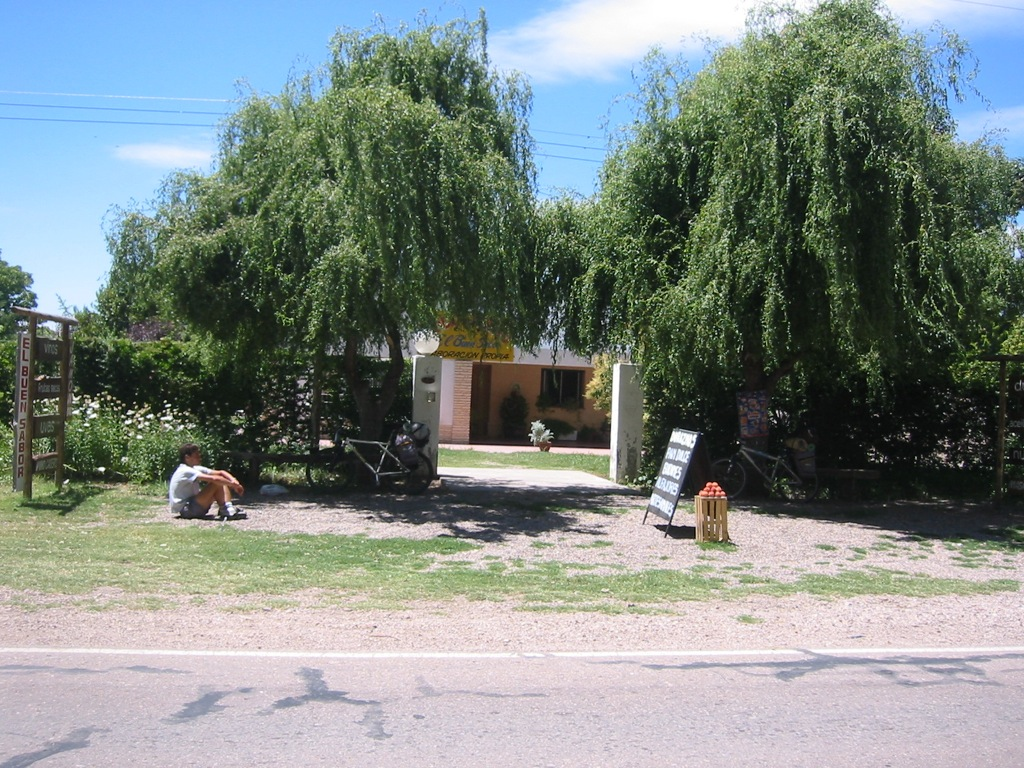
\includegraphics[width=300px]{images/Mendoza_0249.jpg}\\
\textsc{Frutado desayuno camino a San Rafael.} \end{center}

Llegamos a San Rafael, almorzamos muy bien, y decidimos salir para Mendoza en
esa misma tarde porque no encontramos mucho por hacer all\'i. Ten\'iamos
alt\'isimas expectativas, pero pocos fueron los kil\'ometros que las cubrieron
(el ca\~n\'on del Atuel, menos de la mitad del circuito). En realidad todo
estar\'a excelente pero no tanto como esperaba, y, adem\'as, no ten\'ia ganas de
disfrutar porque prefer\'ia siempre dormir. Pero contentos de terminar esta
primera etapa del viaje, y conocer lo que conocimos y hacer lo que hicimos, sin
da\~nos a la salud. Haber llegado.\\

En Mendoza nos cambi\'o la cara. Culminada con \'exito la primer etapa (sin
quemar combustible para cumplirla) nos esperaba esta maravilla de ciudad. De
nuevo sorpresa pero esta vez de la linda, est\'a todo excelente por ac\'a.
Prolija y limpia, buena onda de la gente y mediana de tama\~no, Mendoza capital
est\'a fabulosa. Dejamos los bolsos en un hostal, y recorrimos descansando ayer
y hoy. Era divertido: no ten\'iamos equipaje sobre la bici, ni subidas ni ripio
bajo las ruedas, \textexclamdown y sin embargo no pod\'iamos pedalear!
\textexclamdown Nos costaba avanzar, a\'un en el cambio m\'as liviano!

Al siguiente d\'ia fuimos a la pile de un club, descansamos toda la tarde. La
ducha fue otra salvaci\'on, nunca me dio asco mi piel sucia pero esta vez\ldots\
\textexclamdown mejor no entrar en detalles!

\textexclamdown As\'i que con la frente de nuevo en alto, ma\~nana encaramos el
cruce de la Cordillera en bici! El primer plan era subir por Villavicencio hasta
Uspallata, cruzar por la Ruta 7 a Chile, y volver a Mendoza en colectivo, pero
decidimos subir todo por la 7, volver de Chile hasta Uspallata y\ldots\
\textexclamdown bajar a Mendoza por los caracoles de Villavicencio! As\'i
integramos ambos caminos. Nos lo sugiri\'o un buen lugare\~no interesado por
las bicis cargadas. Ningunos tontos: \textexclamdown as\'i con bajadas
cualquiera viaja!

Estamos ansiosos por entrar en las monta\~nas.

\section{\textexclamdown Empieza el Cruce!}

\subsection*{S\'abado 8 de Enero}

Salimos de Mendoza a Potrerillos, casi descansados, por la ma\~nana.
\textexclamdown C\'omo nos cost\'o salir de la urbanidad de la capital! Hasta el
cruce con la ruta 7 se hizo mucho m\'as largo de lo pensado: 35~km. Luego
tuvimos otros 40~km hasta Potrerillos, pero se ve\'ia de cortina de fondo la
Cordillera de los Andes y nos acerc\'abamos directamente, as\'i que se sent\'ian
bien distinto. Unas horas pedaleando, y logramos meternos en la cortina.

Paramos en una quinta a pedir agua, y un hombre nos advirti\'o del gran calor,
del gran fr\'io, del gran viento\ldots\ ``\textexclamdown Gracias!''
\textquestiondown Pero qu\'e \'ibamos a hacer? Muchas p\'alidas juntas
acompa\~nadas de pocas soluciones. Adem\'as, era lo aceptado al salir de viaje.
Luego, en un parador de barro a la vera de la ruta, paramos a comer un
salad\'isimo pan casero, riqu\'isimo. El lugar divino, atendido por una familia
que vive de esas muy baratas ventas, todos simp\'aticos, y muy prolijito a pesar
de las diferentes sillas y mesas. Bonito. Risas por una tonta ca\'ida al entrar,
un breve descanso, y a seguir.

Llegamos a la bajada a Potrerillos, y en un kiosquito del pintoresco pueblo me
hice ``fana'' de ``Coca-Cola''. \textexclamdown Qu\'e sabrosa se siente al
necesitar l\'iquidos y energ\'ia al mismo tiempo! La disfrut\'e mucho. Llegamos
cansados, por el atrasado y las subidas de la entrada a la Cordillera. El viento
en contra empieza desde el mediod\'ia. Aprendimos r\'apido este detalle,
\textexclamdown pero nunca logramos levantarnos temprano para evitarlo!

Nos indicaron dos campamentos, quedaban bajando por esa calle del kiosco, que
termina en curva cerrada a la izquierda y puente angosto. Los campamentos eran
pasando este puente, a mano izquierda; a mano derecha y tras unos \'alamos
est\'a el dique. Comenzamos a bajar y tomamos r\'apidamente velocidad,
\textexclamdown al describir la curva y pasar por el puente iba tan r\'apido que
no la pod\'ia controlar! Estaba por entrar en sentido contrario una camioneta,
que al vernos pasar hizo se\~nas de luces. \textexclamdown No vi si con cara de
bienvenida o de pocos amigos!

En el primer campamento no entraba ni una carpa m\'as. No dormir\'iamos ah\'i. Y
el segundo estaba tan vac\'io que despertaba sospechas. \textexclamdown Ni el
due\~no estaba! Pero en frente estaban los bomberos, y nos abrieron la
tranquera, asegurando que el due\~no volver\'ia; la idea nos gust\'o. Los
\'arboles estaban marcados con n\'umeros romanos rojos, tenebroso en la soledad.
Pero era perfecto para acampar: sombra en la ma\~nana, colchoncito de pastos
bajo la carpa, enchufes y luz, parrilla, ba\~nos, una linda mesa de
madera\ldots\ \textexclamdown Pero no hab\'ia nadie! No entend\'iamos porqu\'e
la diferencia de gente entre los dos. Nos fuimos a ba\~nar pero los calefones a
le\~na estaban apagados, as\'i que mientras uno se ba\~naba el otro avivaba el
fuego. Cenamos frutas hervidas sobre la original mesa: un c\'irculo de madera
usado para transportar grandes cantidades de cable enrollado. Y, asustados,
pasamos una linda noche. El hombre nunca apareci\'o.

\subsection*{Domingo 9 de Enero}

Desayunamos algo, y seguimos viaje. El due\~no del campamento era de pocas
palabras, as\'i que a\'un pensamos en qu\'e historia esconde este campamento.
Cay\'o esa ma\~nana y le pagamos los servicios.

Ya bien descansados, nos sent\'iamos como siempre, otra vez. Seguimos hasta
Uspallata por la misma Ruta Nacional N$^\circ$7. Bordeamos un poco el movido
r\'io Mendoza, pasaban raftings r\'apido y nos daban ganas de subirnos, debe ser
muy divertido. Con monta\~nas cada vez m\'as altas, nieve apareciendo en pocos
picos, el r\'io siempre tronando al lado y t\'uneles que atravesar (donde se
encajonan los ruidos de los autos y camiones subiendo, estridentes) el
camino fue muy entretenido. Me acuerdo que le contaba a Ezequiel de c\'omo en
los t\'uneles el viento tambi\'en se encajona y lo acelera a uno, una
sensaci\'on emocionante y rara, pero esta vez no atravesamos ni un t\'unel con
buen viento, \textexclamdown todo lo contrario! En alguno nos cost\'o mucho
avanzar.

Unos kil\'ometros antes de Uspallata vimos el cementerio, tendido en la ca\'ida
de una monta\~na. Nos acercamos a las flores para ver c\'omo las manten\'ian en
semejante clima y, claro, eran pl\'asticas. Todas flores de colores, en todas
las tumbas, le daban un toque alegre.

Despu\'es encontramos un barcito donde parar a almorzar, estaba lleno de
camioneros, y todos sus veh\'iculos estacionados alrededor. Son de los camiones
m\'as potentes e inmensos, para cruzar los Andes por Mendoza. Ah\'i comimos un
gran s\'andwich (yo guard\'e la mitad en las alforjas porque ya estaba saciado)
y nos quedamos viendo una pel\'icula c\'omica. La pasamos de diez, los paradores
encantan.

Llegamos despu\'es a la ciudad, y nos instalamos en el primer campamento que
encontramos, pero estaba sucio y casi completamente lleno as\'i que pedimos que
nos devuelvan el dinero. Vuelta a poner el equipaje en las bicis, y seguimos
hasta otro: cerrado al p\'ublico por un festival folcl\'orico. Pens\'abamos
dormir en alg\'un parquecito alquilado (``arrendado'') de una quinta, pero no
encontr\'abamos con qui\'en hablar.

Terminamos preguntando en una iglesia, donde despu\'es de una linda misa y de
idas y venidas de se\~noras a dirigentes y a curas, nos dejaron dormir en la
galer\'ia techada que tienen. \textexclamdown Ni la carpa ten\'iamos que armar!
El piso duro no molest\'o para el buen sue\~no, aunque mi compa\~nero no pudo
decir lo mismo. Los curas y viejas que dirigen divinos, nos despidieron de muy
buena onda, ofreci\'endose para lo que necesit\'aramos. Pensamos que era bueno,
adem\'as, ahorrar los \$12; qu\'e incre\'ible como pasa a otra dimensi\'on el
uso de la plata al viajar as\'i. Yo cen\'e el medio s\'andwich que guard\'e al
mediod\'ia (la mayonesa todav\'ia funcionaba bien), y Eze comi\'o algo liviano.
La noche se hizo para descansar, \textexclamdown nada de andar cocinando!

Nos entretuvimos con una mesa de pool a la que le faltaban algunas bolas
(estaban medio escondidas en un huequito y no las encontramos). Era
divertid\'isimo: uno met\'ia una bola y se escuchaban golpes durante los
siguientes seis minutos. \textexclamdown Despertar\'iamos a toda Uspallata si
segu\'iamos! Tranquilos esta noche, un buen\'isimo descanso. Ac\'a en Uspallata
una curiosidad: hab\'ia rico helado de bananita Dolca en una peque\~na
helader\'ia.

\subsection*{Lunes 10 de Enero}

Ya descansados, casi como nuevos, afrontamos la ruta a Polvaredas.
\textexclamdown Cada vez m\'as Cordillera! Se levant\'o a lo \'ultimo un fuerte
viento en contra, pero 40~km se recorrieron solos entre bajadas y ayudas de la
turbulencia que arrastran los camiones.

En un momento nos pas\'o frenando un grand\'isimo cami\'on chileno, que par\'o
m\'as adelante. Ezequiel se detuvo al lado de su ventanilla y despu\'es el
camionero arranc\'o. Entonces mi amigo se volvi\'o unos metros con una bolsa
naranja grande, sonriendo, y celebr\'o:

\subparagraph{}\label{ssub:camion} --- ``Son buenas para la sed'', me dijo.
\textexclamdown Mir\'a todas las mandarinas que nos dej\'o!\\ \hangindent=1.6cm

La bolsa estaba un tercio llena, as\'i que al sol de esas horas de la siesta
disfrutamos varias, y dejamos otras tantas a la vera del camino. Ten\'ia raz\'on
el conductor: son buenas para la sed. Era una zona donde el r\'io cav\'o un gran
ca\~n\'on y pasa muy por debajo del nivel de la ruta, un lugar precioso y lleno
de distintos colores. Un d\'ia de viaje espectacular, bajo un sol radiante.

Al llegar a Polvaredas era temprano, as\'i que paramos a almorzar. Un gendarme,
luego de explicaciones sobre la canalizaci\'on de los vientos para que siempre
desde el mediod\'ia corra en ese sentido, nos indic\'o un paradorcito donde
comer algo. Charlamos un rato con la due\~na del lugar, tambi\'en le interesaba
escuchar nuestra historia.

A diferencia del sur ac\'a hay poco y nada de mochileros, y llaman f\'acilmente
la atenci\'on. Dicen que es m\'as f\'acil ser ayudado al viajar en bici, porque
los que salen a dedo son vistos como ``hippies'' o m\'as vagos, y la gente no se
solidariza tanto. Nos levanta mucho el \'animo el inter\'es de la gente, nos
llena de voluntad para seguir.

Luego del s\'andwich en este c\'alido parador seguimos a Punta de Vacas, donde
unos gendarmes nos dieron un papel para salir del pa\'is, y para dormir nos
ofrec\'ian una edificaci\'on abandonada, muy oscura y sucia, que ahora usan de
estacionamiento. La otra opci\'on era que caminemos a la vera de un r\'io
perpendicular a la ruta, pero despu\'es de unos 20 minutos de empezar a hacerlo
vimos un cartel que indicaba tres horas (\textexclamdown !) de caminata hasta el
primer campamento, y ya era el atardecer. O no ten\'ian idea del camino (andar
en bici por ah\'i era imposible) o no entend\'ian nuestro viaje, pero volvimos a
Punta de Vacas a tomar una gaseosa para poder seguir hasta Penitentes. El viento
en contra ya nos estaba agotando, es lo que m\'as cansa.

En Punta de Vacas caminamos por los pocos lugares que hay, hasta que encontramos
un contenedor abierto, con un cartel que indicaba que se trataba de un barcito.
Era una preciosura. Al abrir la angosta puerta de doble hoja se entra a una sala
tan larga, angosta y simple como un contenedor puede llegar a ser. Dos personas
charlaban tras una barra y miraban televisi\'on, solos. Cinco mesas
(rectangulares, redondas y cuadradas, ni una similar a la otra) ocupaban el
espacio restante, cada una con sillas de diferentes tipos. Eran en realidad
cinco tipos de sillas, pero mezclados entre las diferentes mesas.
\textexclamdown Una desprolijidad que parec\'ia minuciosamente acomodada!
Pedimos una Sprite de litro, y trajo adem\'as dos vasos de vidrio, cotidianos de
casa de familia. Luego nos tom\'o la foto que le pedimos; es gracioso ver
nuestra posici\'on: tirados sobre las sillas, acostados como si fueran
reposeras, inm\'oviles, forzando la dif\'icil sonrisa mientras apunt\'abamos con
la cara a la c\'amara. Tomamos la botella, nos quedamos un rato m\'as con las
piernas quietas mientras afuera el viento sonaba, y seguimos hasta Penitentes.
Fort\'isimo viento, restaban pocos kil\'ometros pero nos llevar\'ia mucho tiempo
recorrerlos.

Paramos metros antes de Penitentes, en la casa de un vago divino que viv\'ia al
lado de la ruta, con la tranquilidad del pe\'on de campo. Nos ense\~n\'o mucho
de la zona, y nos se\~nal\'o una hoster\'ia donde parar. Ten\'ia adem\'as un
museo de cosas naturales levantado por \'el mismo. Ah\'i vive todo el a\~no, en
medio de la monta\~na, y su \'unica compa\~n\'ia es un guardi\'an y obediente
perro. Tiene electricidad generada por un grupo electr\'ogeno que usa poco.
Prefiere encender una l\'ampara a queros\'en antes que arrancar el motor en
invierno. Muy simple. Nos contaba que de chico sub\'ia con su moto (una Puma),
por el camino de Villavicencio hasta La Cruz, y se tiraba luego con el motor
apagado a dibujar las curvas. \textexclamdown Se le iluminaban los ojos, y
todav\'ia no entend\'iamos lo divertido que puede llegar a ser! Nos volvi\'o a
asegurar, al preguntarle incr\'edulos, que son 365 curvas, ``s\'i se\~nor''.

Paramos en Hotel Ayel\'en, y nos indicaron la Hoster\'ia Ayel\'en, pues no nos
encontraron el suficiente acento alem\'an como para recibirnos. Qu\'e bueno
compartir una cena con ellos, extranjeros de todas las edades prepar\'andose
para escalar el Aconcagua, o gente que ya estuvo intentando y tal vez llegaron,
y estar\'ian contando sus periplos.

No contentos con esto, en la Hoster\'ia nos mandaron a la Guarder\'ia, donde
paraba una familia de pintores y alba\~niles por un trabajo provisorio. As\'i
que por \$10 ten\'iamos habitaci\'on compartida: la m\'as alta de toda la
hoster\'ia y con vista al r\'io (no a las pistas de esqu\'i). Nos duchamos --el
remedio instant\'aneo contra el cansancio y fr\'io que provocan la suciedad-- y
cenamos un lomo completo mirando (esta vez s\'i) a las ahora verdes pistas de
esqu\'i.

Descansamos muy bien.

\subsection*{Martes 11 de Enero}

La ma\~nana del 11 recorrimos poquito las pistas a pie, para salir a la siesta
hacia el Puente del Inca; ya se ve\'ian sus construcciones desde la monta\~na.
Nos distanciaban 8~km de viento en contra, f\'aciles a paso lento. Paramos en el
cementerio del monta\~n\'es, es emocionante. Gente de todo el mundo muerta en
las monta\~nas, con placas llenas de honores sobre tumbas decididamente
rudimentarias.

Al llegar al Puente cruzamos para conocer, caminamos por el viejo hotel derruido
y la capilla, muy interesante y bonito. Fue un d\'ia tranquilo para descansar
piernas y traste, que ven\'ian sufriendo los kil\'ometros que, sino, contin\'uan
acumul\'andose.

Paramos en un camping de por ah\'i, por \$0,50 la due\~na de la casa (en su
patio era el ``campamento'') nos permit\'ia usar la hornalla para cocinar
polenta con leche. Le agregamos salsa, y comimos en nuestra mesa desde la ollita
de aluminio. El fuerte viento la enfriaba tan r\'apido que nos apuramos a comer,
\textexclamdown nos terminamos atorando! \textexclamdown Y para colmo no
llegamos a saciarnos! Qu\'e angurrientos, tuvimos que esperar un rato para poder
acostarnos.

Ducha caliente, a secar el ba\~no, y a dormir pl\'acidamente hasta la siguiente
madrugada.

\subsection*{Mi\'ercoles 12 de Enero}

Nos levantamos a las 8 para visitar las termas del Puente, que s\'olo hab\'iamos
visto. Pasamos media hora relajados en las piletas, nos acostumbramos
r\'apidamente al fuerte olor a minerales. No nos quedamos m\'as porque empezaba
a llegar turismo e incomodaba. Encontramos a un alem\'an en la misma que
nosotros, y mientras nos vest\'iamos le elogiaba su pa\'is pero, sin aceptar
mis palabras, no dejaba de halagar a la Argentina. ``Estando aqu\'i no hay mucho
que a\~norar de Alemania'', explicaba en ingl\'es. Qu\'e lindo, viajar.

Ten\'iamos planeado quedarnos a descansar otro d\'ia en la zona pero\ldots\
\textexclamdown ya conocimos casi todo! Este d\'ia seguimos para Las Cuevas,
pasando por uno de los puntos m\'as atractivos del viaje: el cerro Aconcagua.
Las nubes lo tapaban as\'i que lo imaginamos graaande graande. Ahora tengo otra
excusa para volver a Mendoza: ``\textexclamdown no vi su cumbre!''

Tipo 11 el viento en contra nos empez\'o a frenar, alrededor del mediod\'ia
llegamos y paramos en Las Cuevas, donde ahora s\'i pasar\'iamos el d\'ia de
descanso. Nos metimos y recorrimos, sorprendidos, toda la superficie de una
proveedur\'ia antigua abandonada y derruida. Luego tomamos un gordo chocolate
caliente en la proveedur\'ia antigua de al lado, acompa\~nado con galletitas
dulces y de agua. Un estilo muy alem\'an me pareci\'o el de estos lugares.
Nos atendi\'o una se\~nora de unos setenta a\~nos, ten\'ia un restaurant hermoso
con decoraciones de monta\~na.

Ahora s\'i har\'iamos noche ah\'i, pero\ldots\ \textexclamdown est\'abamos tan
cerca del paso internacional! \textexclamdown Desde ah\'i se ve\'ia el inicio
del t\'unel Cristo Redentor y todo! Nuestro error fue no subir a la imagen del
Cristo por el camino viejo, pues a la 1 de la tarde ya est\'abamos esperando la
chatita que nos atravesar\'ia por el t\'unel (se proh\'ibe, acertadamente,
hacerlo a ciclistas). Mientras esper\'abamos, un gendarme nos indicaba que
nuestras banderitas argentinas no deben lavarse: cuando no dan m\'as, se
cambian. La ansiedad por conocer nos mata continuamente, no podemos estar
quietos. Pasar al otro lado fue un tr\'amite sorprendentemente r\'apido y
f\'acil. Tanto, que olvid\'e declarar la c\'amara de fotos y las bicicletas.

El conductor de la camioneta chilena que nos cruzaba nos dec\'ia que tengamos
cuidado al pedalear por Chile, pues ``\textexclamdown hay muchos conductores
argentinos dando vueltas por ah\'i!'' Entre risas se complet\'o el largo
t\'unel, nos despedimos agradecidos. Fue un alivio el cruce porque no
est\'abamos seguros de poder hacerlo.

\begin{center} 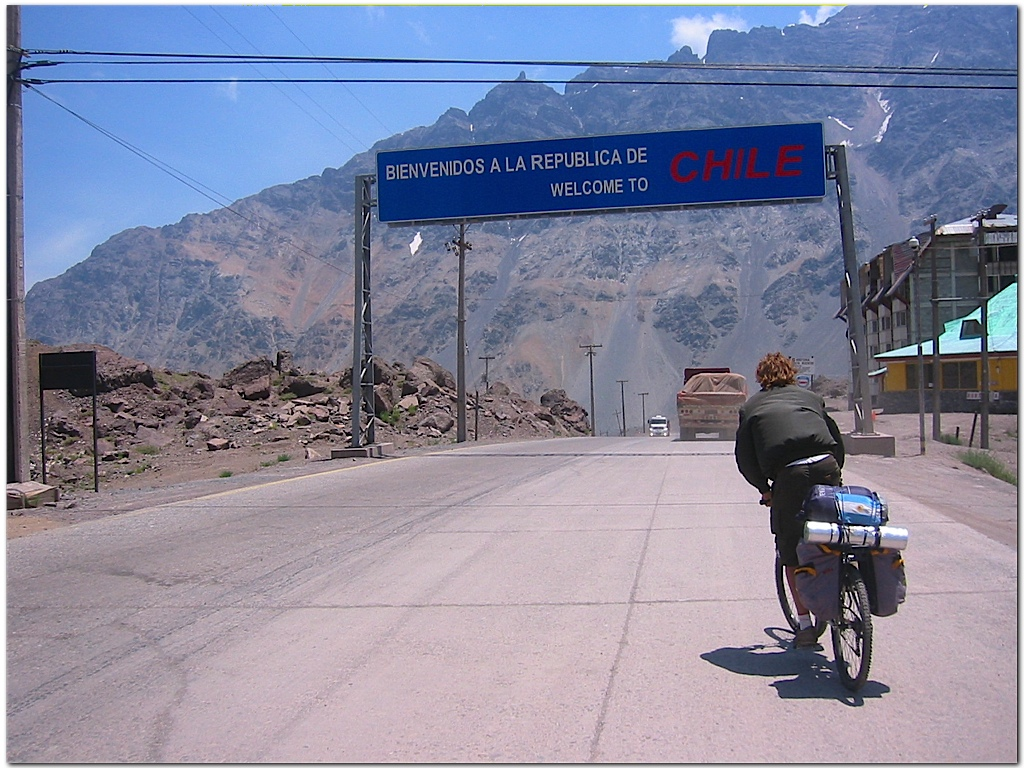
\includegraphics[width=300px]{images/Mendoza_0370.jpg}\\
\textsc{Luego del Cruce, emoci\'on.} \end{center}

Bajamos los caracoles con un fuerte viento en contra, que no nos imped\'ia
adelantar a los camiones. Recordaba de mi primer viaje el olor a frenos quemados
que hab\'ia aqu\'i, pero esta vez el viento nos impidi\'o sentirlo. Baj\'abamos
lagrimeando, entre la emoci\'on y velocidad.

Este fue el momento perfecto del viaje, no puedo describir lo que se siente; fue
espeluznante. A 50~km/h en promedio (entre 70 y 30~km/h) ten\'iamos que apretar
firmemente los frenos para desacelerar la cargada bici, y poder as\'i doblar las
varias y regulares curvas de 180$^\circ$ que conforman este tramo.
Constantemente frenando con dos dedos de cada mano, pedaleando, y zigzagueando.
\textexclamdown Sin ese viento en contra no se si viv\'iamos para contarlo! Las
alforjas empujan fuerte desde ah\'i arriba, se nota mucho. Durante las curvas la
rueda de atr\'as se deslizaba un poco de costado, advirtiendo con un chillido
que no pod\'ia frenar mucho m\'as; eran inyecciones de adrenalina por todo el
cuerpo. Cruzamos en un momento a una pareja en bicis que parec\'ia extranjera,
subi\'endolos. \textexclamdown Tan cargados como nosotros! Los saludamos en el
instante que dur\'o el cruce. No s\'e d\'onde dormir\'ian.

En un momento un cami\'on sub\'ia por su mano contraria, por la l\'inea que yo
iba a usar en mi bajada, de modo de poder abrirse m\'as y no tener que
desacelerar tanto. Por la banquina no lo pasaba, as\'i que pas\'e por mi
izquierda, la parte interna y contraria de la curva, y el hombre pas\'o
tambi\'en por su izquierda, la parte externa. Un cruce \emph{divertido}.

Y en otro momento de esta larga bajada a Los Andes, pero ya en recta,
avanz\'abamos con diferencia de velocidad sobre un cami\'on que m\'as adelante
aceleraba, despu\'es de curvas. Vi que ven\'ia otro cami\'on en sentido
contrario, no lo podr\'ia adelantar; pero quien ven\'ia de frente se abri\'o
cuanto pudo hacia su derecha, y mediante se\~nas con su mano indicaba que nos
dejaba paso al medio. Levant\'e mi mano agradeciendo, y aceleramos pasando por
el medio de los dos camiones: uno bajando, el otro subiendo, y nosotros por el
medio. Emocionante, y peligroso.

La ruta ten\'ia varios cortes por repavimentaci\'on, donde quedaba calzada
\'unica. Al llegar a uno, pasamos justito antes de que cerraran el paso para
permitirles lugar a quienes ven\'ian en sentido contrario, previa autorizaci\'on
del operario, quien avis\'o por handy: ``cruzan tambi\'en dos bicicletas''.
Avanz\'abamos r\'apido por la calzada en buenas condiciones; a nuestra izquierda
ten\'iamos una peque\~na e irregular banquina, y a la derecha una continua
monta\~nita de piedras sueltas que usar\'ian para asfaltar. Porque
demor\'abamos, permitieron el paso de veh\'iculos. \textexclamdown Ver a un
cami\'on subiendo por nuestra misma senda no era de lo m\'as c\'omodo!
Desaceleramos, cruzamos a la calzada que estaban arreglando, y dejamos paso a
quienes sub\'ian. Qu\'e f\'acil es en bicicleta.

Llegamos a Los Andes. Ah\'i nos sugirieron preguntar por Eric, un veterinario
holand\'es, que hizo brutos viajes en bicicleta, y aloja gratuitamente a sus
``colegas''. En la plaza central de un hermoso boulevard muchos nos miraban
sorprendidos y se acercaban a hacer preguntas, pero s\'olo dos de ellos supieron
indicarnos la casa de este hombre. Como justo estaba de viaje tuvimos que buscar
otro lugar donde dormir.

Nos mostraron un hotel ``barato'' pero era hotel, as\'i que seguimos viaje para
ver si encontr\'abamos campamentos. Todav\'ia ten\'iamos horas de luz. Pasamos
San Felipe, luego dos campamentos que no aceptaban d\'olares y me enojaron
mucho, pues quer\'ia parar. M\'as adelante nos indic\'o un hombre con ojos muy
rojos un lugar donde parar, con gestos en el aire nos indicaba:

\subparagraph{}\label{ssub:manan-tiales}
--- Van a ver el cartel: manan-tiales. S\'i: \emph{\textexclamdown
manan-tiales!}\\

Y como todos los chilenos que nos ayudaron, repet\'ia las indicaciones a seguir.
\textexclamdown Era muy gracioso!

Llegamos por fin al prolijo lugar cercano a Panqueue, atendido por una muy
amable y humilde familia. Mientras esper\'abamos al padre, dos chiquitos nos
llenaban de preguntas, estaban admirados. No lo pod\'ian creer: nunca hab\'ian
visto personas viajando en bicicleta. Cuando el hombre lleg\'o, no ten\'iamos
que actuar la cara de cansados, tambi\'en la oscuridad hablar\'ia por nosotros.
Les contamos la historia de este d\'ia, que empez\'o temprano en la ma\~nana en
el ya lejano Puente del Inca, pero no conoc\'ian Argentina. ``Es un lugar muy
lindo\ldots'', y parec\'iamos de otro planeta.

No s\'olo no tuvieron problemas en dejarnos pasar, sino que adem\'as nos
hicieron sentir muy c\'omodos. Ped\'ian s\'olo dos d\'olares por cada uno
contando carpa. El hombre nos mostraba las instalaciones: la pileta de agua
congelada de manantial que podr\'iamos usar ma\~nana, los ba\~nos (ya era hora
de apagar los calefones, pero esperaron a que nos instal\'aramos y
ba\~n\'aramos), las parrillas, etc. Vimos que era un lugar muy familiar, estaba
lleno de autos y tal vez por eso se sorprendieran los chicos por nuestras bicis.

Personas muy serviciales, \textquestiondown c\'omo no voy a enojarme cuando
alguien generaliza diciendo ``los chilenos son antip\'aticos''? Es claro que los
primeros que encontr\'aramos no nos iban a ayudar como necesit\'abamos, pero
depend\'ia de seguir buscando el encontrar buenas personas.

Este d\'ia completamos 125~km y pasamos por alto tres noches (en Puente del
Inca, en Las Cuevas y en Los Andes). Nos cost\'o encontrar un lugar pero
lleg\'o, asegur\'andonos un buen descanso y linda cena. Charl\'abamos de pasar
el siguiente d\'ia en la pileta, descansando, pero al mediod\'ia no pod\'iamos
estar parados en Chile, \textexclamdown hab\'ia que seguir conociendo! Y de
nuevo acortamos d\'ias continuando viaje.

\subsection*{Jueves 13 de Enero}

Bien descansados, la siguiente tarde nos recibi\'o en la ruta, llena de curvas
al principio, con prolij\'isimos montes frutales alrededor, gran sol y cielo
azul. Pero luego el viaje se torn\'o mon\'otono, con suaves sierras y una recta
autopista que se ve\'ia a lo lejos seguir\ldots\ Eso es malo porque parece que
no se avanza, el paisaje parece nunca cambiar. Almorzamos panes caseros y
bananas frente a un comercio del camino, atendido por una mujer que relataba
todos sus problemas al justificar su precio del d\'olar. Me dio un poco de mal
humor.

Ah\'i mismo arreglamos una pinchadura, y un joven nos indic\'o que m\'as
adelante hay un t\'unel prohibido para ciclistas, pero no ten\'iamos otra ruta
alternativa hacia el Pac\'ifico. El problema era si el t\'unel ten\'ia 1~km, 8
como nos dec\'ia el chico, o menos de 1 como otro nos dijo. Ni 8 ni menos de 1,
pero se nos hizo muy corto por el miedo de que fuera verdaderamente largo. Los
autos nos tocaban bocina con raz\'on.

Par\'abamos en La Calera por el viento en contra que nos cansaba, pero era feo y
ni campamento ni hoster\'ia hab\'ia. Paramos a tomar un helado para seguir luego
viaje, pero no nos aceptaban pagar en d\'olares. Una joven madre escuch\'o el
problema y se ofreci\'o a cambiarnos \$600 chilenos por un d\'olar. Linda
actitud.

En ruta a Quillota y luego del helado, pinchamos una rueda trasera sobre un
puente en curva. Una camioneta argentina nos vi\'o arregl\'andola y fren\'o,
baj\'o y se ofreci\'o a llevarnos, pues compart\'iamos destino, Vi\~na del Mar,
a unos 60~km. Pero no cumplir\'iamos con la gran meta, as\'i que decidimos
(Ezequiel decidi\'o, en honor a la verdad) agradecerle y seguir pedaleando
despu\'es del arreglo. El buen hombre se subi\'o sonriendo a la camioneta, y
sigui\'o luego de felicitarnos. Otra buena actitud.

Seguimos acumulando cansancio hasta Quillota, pero era igual, m\'as desprolija y
parec\'ia menos segura, as\'i que, luego de cambiar d\'olares, tipo 7~pm paramos
a comer un gran s\'andwich. Preguntaba la cocinera: ``\textquestiondown Lechuga
picada o de hojas completas?'' \textexclamdown Atenci\'on de lo m\'as
personalizada luego de ganarnos su simpat\'ia! Al principio se enojaba porque
quer\'iamos entrar las bicis, pero le contamos el viaje y que quer\'iamos comida
r\'apida, que necesit\'abamos cuidar todo lo que ten\'iamos (literalmente,
todo), y entonces cedi\'o. Nos sirvi\'o en platos distintos, el m\'io era
amarillo y de ni\~nos, como de juguete. \textexclamdown Ezequiel se
re\'ia cuando saqu\'e la c\'amara para recordarlo! Mis fotos no sirven para
portarretratos ni para concursos, tendr\'e que aceptarlo.

No nos qued\'o otra que seguir a Conc\'on, donde empezar\'ia la costa pac\'ifica
chilena. 90~km este segundo d\'ia, alto promedio en Chile. \textexclamdown En
dos d\'ias cruz\'abamos la Cordillera desde Puente del Inca, y lleg\'abamos al
Pac\'ifico! Tuvo su precio pero tambi\'en su recompensa. El cansancio f\'isico
acumulado es similar al de San Rafael, pero la buena onda ps\'iquica de por fin
estar en los paisajes que esper\'abamos y de la meta (no circuito sino
\emph{viaje}) nos permit\'ia seguir sin perder la sonrisa.

Llegamos a Conc\'on ya de noche. Sobre un puente ped\'i foto a Ezequiel, pero no
quer\'ia sacarla porque no mostraba ni el momento, ni el lugar; no ``dec\'ia''
nada. Pero el recuerdo es lo que para mi vale; por eso me cuesta entender que
mis amigos o hermanos se aburran al mostrarles \emph{todas} las fotos. S\'olo yo
puedo recrear la escena en mi cabeza partiendo del retrato, ya que lo viv\'i.

La gran pregunta era ahora d\'onde pasar esa noche. Una chica de Santiago de
Chile nos dijo que acampaba bajo ese puente, pero es ilegal y si los
sorprend\'ian los echaban. Quer\'iamos comodidad, \textexclamdown era casi el
fin de nuestro viaje! Toc\'abamos puertas para alquilar una habitaci\'on o un
pedazo de pasto pero no nos hac\'ian caso, ya estaba oscuro para pedir ese tipo
de ayudas. Info tur\'istica cerrada y hoteles caros promet\'ian jodernos la
noche de merecido descanso. Preguntando llegamos a una hoster\'ia no muy cara, y
excelente. Ducha, inodoro que necesitaba urgentemente (y que siete cadenazos no
pod\'ian terminar con su trabajo), tres camas (una grande y dos de plaza y
media), m\'as frazadas y {\small TV}, nos daban el descanso y respiro que
necesit\'abamos. Los U\$S 14 m\'as disfrutados del viaje. Un reconfortante
ba\~no y a comer algo, con un leve mareo por hambre y cansancio, que a la vez me
hac\'ian querer salir a festejar y quedarme a dormir.

Caimos en un lugar barat\'in, que por resultar ser de argentinos no jodieron con
la moneda internacional que nos quedaba. La joven pareja nos prepar\'o buenos
s\'andwiches con un chimi-churri ``lo m\'as argentino posible'', y palta, muy
buena. Despu\'es charlamos de lo lindo, nos ense\~naron muchas cosas sobre
c\'omo movernos en Chile. Nos felicitaron por el viaje, y quedamos en volver a
almorzar ma\~nana. Nos ofrec\'ian su casa para dormir, nos ofrecieron internet.
``\textexclamdown Gracias!''

\subsection*{Viernes 14 de Enero}

Hoy nos despertamos temprano para aprovechar el desayuno del hotel, nos tiramos
otro rato a dormir, nos duchamos otra vez\ldots\ \textexclamdown y eran las 12!
\textquestiondown C\'omo parar a almorzar en un lugar conocido, si no
conoc\'iamos la costa chilena?

Comimos unos poderosos alfajores de dulce de leche, y recorrimos toda la
costanera hasta Valpara\'iso. ``La foto'' del viaje fue en una playa de Vi\~na
del Mar; salen tambi\'en los protagonistas secundarios, esos alfajorzotes, y el
oc\'eano, que no se nos ocurri\'o tocar para comprobar que es tan fr\'io como
dicen. La excusa es esta vez para volver a Chile.

Encontramos mucha belleza en esta costanera, donde el mar se ve hermoso con ese
color turquesa, y esas piedrotas angulosas que lo decoran. Como balneario no
deben ser buenos, pero s\'i para ver. Es una ruta com\'un, mano-contramano, que
bordea la serpenteante costa, separada del mar s\'olo por pocos metros de altura
y un guarda riel. Se disfrut\'o much\'isimo de estos descansados 25~km. Una
familia vio nuestras banderas argentinas y nos gritaban saludando y alentando.
Vi muchos Subaru, pero pocos del Turbo, los deben elegir por la nieve y su
tracci\'on integral. Un Porsche en un restaurant coqueto que daba al Pac\'ifico
adornaba el estacionamiento.

Helados de por medio, anduvimos hasta Valpara\'iso, donde preguntamos por la
casa de Pablo Neruda. \textexclamdown Est\'abamos tan cerquita, pero para llegar
hasta all\'a arriba ten\'iamos que desviarnos tanto! Hasta esa avenida de arriba
caminamos diez cuadras de subida muy empinada, con bicis cargadas. Antes tuvimos
que llegar al inicio de esa subida, describiendo entonces una ``V'' corta. Las
cuadras son figurativas para nuestro sistema, porque pasamos s\'olo dos o tres
cruces de calle en esa distancia.

La casa es un sue\~no. Cinco pisos de poca superficie cada uno, habitaciones de
tama\~nos raros, decenas de naturalezas muertas en cada habitaci\'on y pasillo,
adornos de todo tipo, escaleras de diferentes formas y alturas, el mar se ve
desde todas y cada una de las muchas ventanas (hasta desde los ba\~nos), y saber
que Neruda ah\'i escribi\'o y am\'o tantas cosas\ldots\ El artista imitaba al
barco desde su casa, porque si bien le apasionaba el mar, no se animaba a
navegar. Menos mal que estaba esta casa tan divina, porque encontramos
Valpara\'iso muy industrial y poco tur\'istico, a diferencia de la belleza que
muestra Vi\~na del Mar\protect\footnote{Recorrimos poco, luego conoc\'i
descripciones inversas.}.

La vuelta a abajo fue monumental, esas diez cuadras de ahora \emph{intensa}
bajada, pero de calle com\'un, con esos saltitos de brea entre los bloques de
cemento, fueron tremendas. \textexclamdown Con dos dedos en cada freno y con los
otros agarrados del manubrio, necesit\'abamos m\'as manos! No lleg\'abamos ni a
frenar bien ni a sostenernos firmemente, pero de hacer una cosa dej\'abamos
totalmente la otra! La rueda de atr\'as pegaba un chillido en cada saltito,
mostrando que ven\'ia agarrada del pavimento como pod\'ia. Las relativamente
pocas bocacalles nos daban un m\'inimo de seguridad.

Y ahora a comer m\'as alfajores y a la terminal, para volver a Uspallata y bajar
a Mendoza, pero por los caracoles de ripio de Villavicencio. Comprobaremos que
las 365 curvas no son exageraci\'on.

\subsection*{Mail enviado desde Santiago de Chile, pocas horas despu\'es:}

As\'i como llegamos a la terminal, nos subimos corriendo a un bus a Santiago,
porque no hay lugar ni para las moscas en los colectivos, mucho menos directo a
Uspallata desde Valpara\'iso. Llegamos a la estaci\'on y todos nos dec\'ian ``no
hay lugar''\ldots\ \textquestiondown C\'omo pudimos ir tan confiados, como si ya
todo estuviera planeado? Plata para volver en bici no ten\'iamos. Si nos
dec\'ian ``tienen que esperar cinco d\'ias'' probablemente tuvi\'eramos que
comer una vez al d\'ia. Pero el hombre nos dio los pasajes, que despu\'es
descubrimos que estaban mal, entonces volv\'i desesperado a su oficina mientras
Ezequiel cuidaba los veh\'iculos.

\subparagraph{}\label{ssub:Valparaiso} --- Bueno chicos, \textquestiondown pero
ustedes se quieren ir ahora? \\ --- \textexclamdown S\'i, claro! \textexclamdown
Ahora! \\ --- \textquestiondown Ahora, pero ya en este preciso momento? \\ ---
\textexclamdown S\'i, cuanto antes puedan mejor! \\ --- Bueno, entonces
\emph{ya} vayan al colectivo de la plataforma 7 porque los est\'a esperando, les
digo que se demoren 5 minutos. \\ --- \textexclamdown Pero tenemos las
bicicletas! \textexclamdown Todav\'ia no las desarmamos! \\ --- No importa, las
metemos en las bodegas como est\'en.\\ \hangindent=1cm

Corrimos al bus, nos ayudaron a meter las bicis, subimos y arrancamos. No s\'e
como llamar a eso pero les aseguro que as\'i estaba planificado, parec\'ia que
estaban esperando a estos dos viajeros para irse a Santiago y combinar hasta
Uspallata.

En el viaje \'ibamos pensando: ``\textquestiondown Qu\'e pas\'o?'' Est\'abamos
confundidos, no sab\'iamos si hab\'iamos hecho bien en subirnos, mir\'abamos y
revis\'abamos los pasajes, nos pregunt\'abamos si nos habremos olvidado algo
en las corridas\ldots\ \ \textexclamdown Fue raro! Pero funcion\'o como
esper\'abamos.

Al anochecer, al entrar en la Capital ve\'iamos c\'omo son sus colectivos de
l\'inea, nada lindos. Todos viejos, todos iguales, todos amarillos con grandes y
negros n\'umeros cuadrados a los lados que indican la l\'inea. Acostumbrado a
los colectivos porte\~nos, que muchos son un monumento art\'istico, se notaba el
cambio. Y ac\'a estamos, en la gran ciudad, esperando se hagan las 8 am para
salir a Uspallata en un ``R\'apido''.

Comimos en plato y con cubiertos, \textexclamdown ni me acordaba como se usaban!
Los del restaurant, divinos. Era sobre un boulevard muy lindo en
construcci\'on, lleno de conos y carteles naranjas. Una mujer cercana a los
sesenta a\~nos, luego de felicitarnos fervorosamente nos sugiri\'o cenar ah\'i,
y no le err\'o: \textexclamdown hasta las bicis al lado de la mesa nos
permitieron! Era demasiado. Era un lugar muy grande con muchas mesas, de las que
quedaban dos libres. Todo el restauran se daba vuelta para ver a los dos
delirantes maniobrando las m\'aquinas cargadas, para dejarlas cerquita pero sin
que molestaran al pasillo. Al lograr sentarnos, transpirando de la verg\"uenza,
nos sugirieron que cambiemos de mesa para estar m\'as c\'omodos. ``As\'i est\'a
bien\ldots'' Pero con \'animos de ayudarnos nos levantaron y llevaron a otro
lugar, de verdad m\'as c\'omodo. Escuchaban con atenci\'on sobre el viaje, todos
se sorprenden y nosotros tambi\'en porque ya pasamos los 700~km recorridos.
\textexclamdown Es que hicimos 230~km en Chile, en dos d\'ias! Vamos a un
promedio de m\'as de 60~km por d\'ia desde que salimos, mi traste ans\'ia un
sill\'on donde apoyarse.

Nos vemos en pocos d\'ias, luego del festejo en Mendoza de haber \emph{cruzado
la Cordillera} a pedal. Nos morimos de risa por el tono con que decimos
``\emph{cruzar la Cordillera}''. \textexclamdown Suena gordo y lo exageramos a
prop\'osito!

Ac\'a el argentino que atiende el cyber (que no para de decir ``boludo'',
necesita volver a su pa\'is) nos dice que no hay fernet por Chile, as\'i que nos
sacaremos las ganas en Argentina. Estamos totalmente libres de toxinas despu\'es
de dos semanas transpirando y tomando agua de monta\~na. \textexclamdown Pero no
ser\'a por mucho tiempo!

A medianoche salimos del cyber, y, paseando por una plaza central, nos
encontraron dos chicas de unos 25 a\~nos, que caminaban junto a un peruano de
similar edad, completamente ebrios. Empezaron a charlar, se re\'ian, hac\'ian
chistes\ldots\ \textexclamdown Hac\'ian preguntas, y no dejaban tiempo
suficiente para que respondi\'eramos! Ezequiel no puede recordar lo siguiente
sin re\'irse: el hombre quer\'ia que dij\'eramos que ellos (Per\'u) eran los
m\'as grandes jugando al f\'utbol. Nosotros le fundament\'abamos porqu\'e no lo
quer\'iamos decir pero \'el insist\'ia, todo lo que quer\'ia era escuchar eso.
Sin mucho sentimiento le asentimos: ``s\'i, ustedes son los m\'as grandes''.
\textexclamdown Despu\'es de todo era irrelevante! Al escucharlo dibuj\'o
sonrisa, se qued\'o tranquilo, y se fueron. \textexclamdown Simplemente lo
quer\'ia escuchar! Un encuentro raro y divertido. Ezequiel nunca lo recuerda sin
re\'irse.

Hablando de sin-sentidos, qu\'e guachos somos varios argentinos, despu\'es ``nos
queremos llevar bien con `los chilenos' ''. Un verdulero de Uspallata nos dijo,
concluyendo entre otras cosas: ``\textexclamdown y lo bien que los tratamos, a
los hijos de p@\#\&!'' \textquestiondown No se dan cuenta? Y la mujer del
restaurant de Conc\'on, que ``nos odian porque\ldots\ \textexclamdown somos
mejores!'' Y sonrisa. Cara-rotas es poco decir. Brutos.

\textquestiondown Cu\'antos chilenos nos odian? \textquestiondown S\'i?\\
\indent \textquestiondown Y qui\'enes, por ejemplo? \textquestiondown S\'i?\\
\indent \textquestiondown Y porqu\'e? Empezar por casa es m\'as f\'acil que
justificar el maltrato, me parece.

Del encuentro con los tres muchachos de fiesta seguimos paseando por el Centro.
Pasamos por edificaciones hermos\'isimas, muy bien iluminadas, imponentes,
tendr\'an una historia digna de conocerse.

Caminamos por una linda y prolija peatonal donde, tom\'abamos un helado parados
con las bicis entre las piernas, para cuidarlas. Pasaron dos o tres hombres de
unos 40 a\~nos que hablaban en ingl\'es, no se notaba que hab\'ian tomado sino
por c\'omo hablaban. O tal vez lo hac\'ian por la libertad de saberse en la otra
punta del mundo donde no todos hablan ingl\'es. Pero empezaron en voz alta:
``\'estos son verdaderos ciclistas, nosotros somos gallinas''. Yo me di vuelta,
sorprendido, con una sonrisa que les habr\'a mostrado que los escuchaba. ``Eso
es viajar en bicicleta: con los bolsos, la carpa, la bolsa de dormir\ldots\ \
\textexclamdown Como nosotros cualquiera es ciclista!'' Lo hac\'ia de muy buen
modo, con mucho humor, ten\'ia ganas de contestarles para empezar a charlar,
pero as\'i como aparecieron a mirar las alforjas y banderita se volvieron a ir.

Nos dec\'ian lo mismo que los viajeros de San Rafael, pero ahora no podemos
pensar que fuera por compromiso o para ayudarnos durante una \'aspera subida,
empapados en transpiraci\'on como aquella vez. \textexclamdown Era su
conversaci\'on! Es evidente que no se necesita privarse de comodidades por
d\'ias para ser ciclistas. Pero aparentemente a ellos les interesaban los viajes
largos y les gustar\'ia hacer uno, tal vez no se animaran a decir ``chau vieja,
vengo en tres semanas''. Sino, \textquestiondown para qu\'e decirlo?
\textexclamdown Con decir ``a estos dos les chifla el mo\~no'' bastaba! O
simplemente dos tipos que tienen ganas de pedalear, ni locos ni Ciclistas con
may\'usculas. No hay que quedarse, hay que salir, cada uno en la medida que
pueda y quiera. Pero hacerlo cuando se puede.

Otro pensamiento para m\'i raro: una mujer en Quillota no dejaba de pensar que
estamos locos. Le explic\'abamos que no, que era el modo que eleg\'iamos para
conocer. ``\textexclamdown Pero hay que tener ganas, ehh!'', conclu\'ia.
Baldeaba su vereda mientras conversaba. Tomamos de su agua, y seguimos
pedaleando despu\'es de saludar y agradecer. Tal vez sea este tipo de reacciones
las que me llevaron a querer escribir los relatos. Mostrar la simpleza y
humanidad (no super-heroismo) que hay en nuestras ganas de viajar en bici.

Volvimos a la Terminal de Santiago por ese boulevard tan lindo en
construcci\'on. Tanto desorden provocado por las mejoras, la poca luz, y mi
cansancio y sue\~no, hac\'ian que empiece a enfocar dificultosamente. Sin
embargo, me acuerdo como si una cinta lo estuviera proyectando sobre mi frente.
Parec\'ia de mentiras, parec\'ia un jueguito de computadora. En la capital
chilena, pedaleando en contramano (no hab\'ia tr\'ansito) a trav\'es de
m\'aquinas amarillas, conos rojos luminosos, carteles de diferentes colores,
tipograf\'ias y modos de colgarlos, gente en la noche de ese Viernes y madrugada
de S\'abado\ldots\ Esos momentos tan especiales hacen que vayamos muy r\'apido,
ya que no hay grandes distancias por recorrer. Entonces yo lo segu\'ia a mi
amigo, que con sus alforjas y banderita flameando era como un se\~nuelo, y me
divert\'ia viendo el paisaje moverse cercano y r\'apidamente. De esos momentos
que se graban en la memoria.

Llegamos a la Terminal, y tuvimos que mostrarle los pasajes al guardia para que
nos dejara pasar. La cierran, pero no para todos. Nuestra noche no se hizo muy
larga: pudimos dormir bien en el piso porque est\'abamos cansados, aunque no
mucho tiempo como necesit\'abamos. Nos despertaban para limpiar, y nos
volv\'iamos a estirar en el suelo. Ni escuch\'abamos cuando quer\'ian
levantarnos, entonces sent\'iamos que nos pateaban con poca tranquilidad en la
planta de los pies. \textexclamdown Al despertarnos ve\'iamos a la se\~nora que
trabaja en la limpieza con cara de pocos amigos, y a los dem\'as viajeros
mir\'andonos conteniendo la risa! La luz del lugar nos volv\'ia a encandilar,
hasta que encontr\'abamos otro lugar y posici\'on donde seguir durmiendo. Lo
hac\'iamos contra las puertas de las boleter\'ias, para que al abrir nos
despertasen y tomar entonces el colectivo de esa madrugada.

\section{Las 365 curvas de Villavicencio}

\subsection*{S\'abado 15 de Enero}

Subimos a nuestro bus despu\'es de embalar las bicis, llegamos a Uspallata
despu\'es de ver toda la ruta que hab\'iamos recorrido, ahora de vuelta y a
trav\'es de la ventana. Pod\'iamos ver en todo el viaje al r\'io y las v\'ias,
que no pod\'iamos apreciar desde nuestro lado al bajar contra la monta\~na. Y
as\'i, mirando la extensi\'on recorrida, dije lo que nunca se me hubiera
ocurrido pensar: ``\textexclamdown hay que tener ganas, ehh!''. \textexclamdown
Pero nunca faltaron! (Casi.)

En Uspallata comimos bien y salimos para Villavicencio, que, a no mucha
distancia de bajada y con poco viento por la zona, promet\'ia ser una frutilla
del postre, un fin de viaje relajado. \textexclamdown El broche de oro!
Villavicencio estaba a 70~km al final (m\'as 50~km a Mendoza capital) pero todo
bajada y sin viento\ldots\ Villavicencio estaba a 70~km con mitad subida, mitad
bajada, y fuerte (el primer d\'ia, pues al final nos tomamos dos para
completarlo) viento en contra. \textexclamdown El clima de viajeros en bici
volver\'ia, nuestro viaje no terminaba! El broche de oro requer\'ia exigencia.

Demor\'abamos la salida. Tomamos helado, paramos en una arboleda\ldots\
despu\'es nos esperaban aridez, sol y condiciones desfavorables para mantener
una velocidad media. Subimos a un promedio de 6~km/h entre el cambio liviano y
caminatas. El viento nos frenaba mientras los serruchos nos quitaban el
equilibrio. En las subidas empinadas la rueda delantera se levantaba al mover
los pedales, impidiendo a la trasera traccionar. Tomamos toda el agua que no
usar\'iamos hasta Mendoza. \textexclamdown Y todav\'ia no est\'abamos a medio
camino de la Reserva! Peligroso, aunque de vez en cuando cruz\'abamos personas.

Cay\'o la noche, pero la luna estaba creciendo as\'i que hab\'ia luminosidad.
Seguimos por unas eses en subida que recordaban a esa subida de San Rafael:
mientras se piensa que no se puede estar m\'as alto, se sigue subiendo y las
eses se prolongan, y los cerros siguen cortando la visi\'on del camino de
subida\ldots\ \textexclamdown Y charl\'abamos de qu\'e hacer en caso de que se
nos cruzara un puma! ``Hay que hacerse el grande con los brazos, y quedarse
quieto''. \textexclamdown Serenidad es lo que faltaba!

No encontr\'abamos ni donde tirar la carpa hasta una cruz que hay por ah\'i.
(``La Cruz'', un mirador de la pared Norte del Aconcagua.) No entend\'iamos
que fuera un mirador: \textexclamdown tanto tiempo vimos ese paisaje durante la
lenta subida! Era el punto casi m\'as alto antes de empezar la --m\'itica para
nosotros-- bajada de Villavicencio de unos 20~km y 365 curvas. Era de noche y
est\'abamos de verdad cansados, con poca agua y hambrientos. Decidimos no s\'olo
descansar sino adem\'as esperar a que saliera el sol, para deleitarnos de verdad
con esa bajada tan deseada, que en planes ya deber\'iamos haber bajado pero
todav\'ia ni siquiera ve\'iamos.

Mientras arm\'abamos la carpa pasaron dos autos. Hicimos se\~nas a cada uno para
que frenara y por favor calmara nuestra sed. Uno pas\'o despacito mirando, pero
no debe haberse animado. \textexclamdown Estaba oscuro! El segundo, una
``Traffic'' conducida por una joven pareja, fren\'o a preguntar algo y nos
dej\'o dos litros de agua despu\'es de contarles un poco nuestro viaje.
Impresionante. La chica as\'i estaba, impresionada. Nos salv\'o esa noche y el
siguiente desayuno, pero, m\'as que nada, la salud y bienestar para el siguiente
d\'ia. \textquestiondown Qui\'en viaja en auto con una botella de dos litros
atr\'as, llena de agua? Otra casualidad que necesit\'abamos y nos solucion\'o un
importante problema. Eran dos chicos de Capital Federal, que subieron todo sin
saber c\'omo era y\ldots\ \textexclamdown se les hizo largo! No sabemos c\'omo
se les puede hacer largo este camino. Los primeros eran amigos y siguieron
viaje, pero ellos, cansados, pasaron la noche tambi\'en cerca de La Cruz.

Comimos algo, y nos tiramos a dormir. En medio del silencio cordillerano, Eze
pregunt\'o: ``\textquestiondown Qu\'e estar\'an haciendo los muchachos ahora?''
Y tambi\'en empec\'e a pensar en aquello. Era un s\'abado a las 10:30 de la
noche. ``El abuelo'' se estar\'ia ba\~nando para recibir a los dem\'as en su
casa. El ``pelado Queen'' estar\'ia poni\'endose desodorante para caminar al
centro. El ``Otto'' estar\'ia afeit\'andose con la canilla abierta.
\textexclamdown Las cosas cotidianas que cada uno de nosotros hace un d\'ia como
ese a una hora como esa, y que sin embargo nos eran tan lejanas y fuera de la
realidad, que ni siquiera las a\~nor\'abamos! Creo que esa noche mis viejos
estaban de gala en el casamiento de un sobrino. Es rar\'isimo e
interesant\'isimo pensar en esos mundos distintos pero paralelos. Nosotros
est\'abamos echados como nos hab\'iamos echado en una carpa, en una noche
ventosa en el medio de un cerro, habiendo cenado un paquete de ``Melbas'' y un
alfajor ``Milka''. \textexclamdown Habiendo hablado de hacernos los grandes con
los brazos ante la presencia de un puma!

Estos pensamientos no nos impidieron dormir profundamente.

\subsection*{Domingo 16 de Enero}

Nos levantamos a la ma\~nana siguiente, y desayunamos las sobras de la cena
(galletitas ``Melba''). As\'i que muy bien nutridos, a las 9:30am, levantamos
campamento y salimos en las bicis.

\textexclamdown Impresionante! El viento hab\'ia rotado y ya pod\'iamos pasar
los 20~km/h. Despu\'es de un d\'ia a 6~km/h significaba un reconfortante alivio.
No s\'olo eso: a 35~km/h los serruchos nos acalambraban los dedos, y llegamos
hasta la verdadera \'ultima subida. Desde ah\'i empezaban \emph{los caracoles},
de ripio, piedras y marcados serruchos.

Fue divino, \textexclamdown se demor\'o pero lleg\'o el premio! Desde ah\'i
arriba se ve\'ia el suelo de Mendoza, la lejana planicie tras las monta\~nas. La
ruta que tomar\'iamos desde el Hotel Villavicencio a la Capital parec\'ia desde
ah\'i una pista de aterrizaje. Los caracoles son incontables curvas (si uno las
baja) de ripio que pasan por varios cerros, as\'i que tienen variadas formas,
pendientes, y peraltes, a diferencia de los regulares y asfaltados caracoles de
bajada a Chile. \textexclamdown Una deliciosa prueba para los ciclistas! Era
lindo ver c\'omo la bici iba de lado a lado de la senda, mientras uno no variaba
la direcci\'on, as\'i de sinuoso era el camino. Otra vez, \emph{espeluznante}.
Nunca viv\'i algo tan entretenido sobre la bici, por tiempo tan prolongado. Eso
es lo que lo hizo \'unico.

\begin{center} 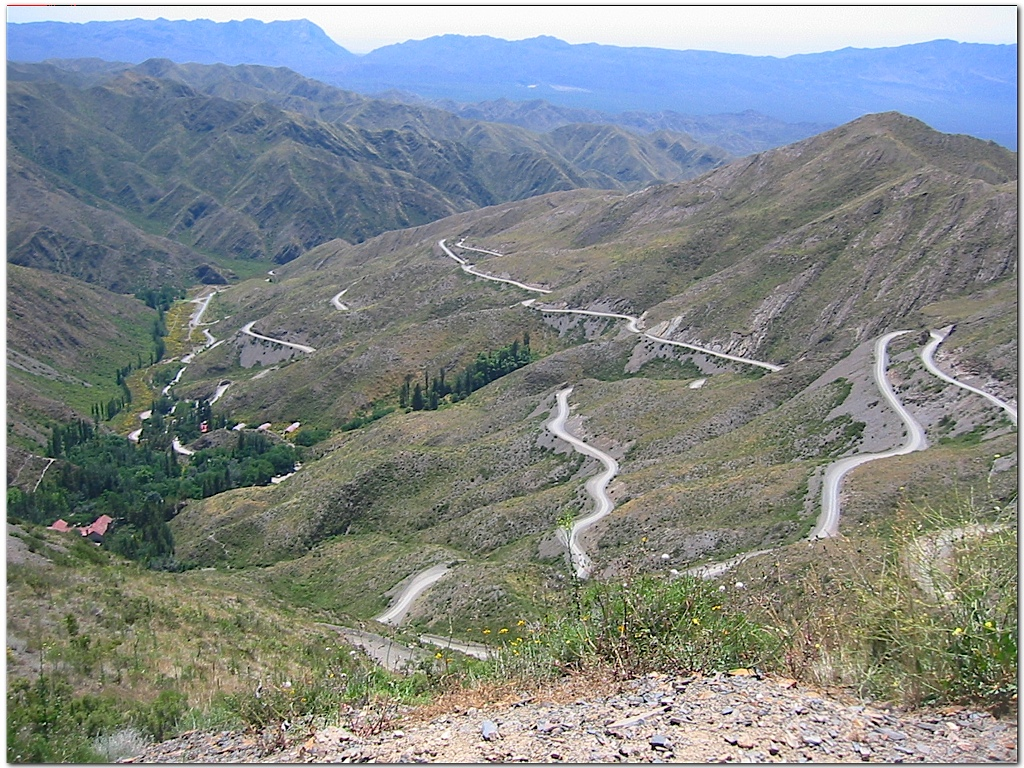
\includegraphics[width=300px]{images/Mendoza_0450.jpg}\\
\textsc{El impredecible camino.} \end{center}

La sensaci\'on de que un motor no nos deja de acelerar, de llegar a 45~km/h a
frenar antes de las (cerradas) curvas --que no se ve c\'omo sigue el camino si
son a la derecha--; la senda all\'a abajo, vi\'endose serpentear y esperando
nuestro paso; el dedo \'indice en los frenos mientras los otros cuatro se
aferran fuertemente del vibrante manubrio; las cubiertas escarbando la tierra
intentando desacelerar\ldots\ pocas veces (por suerte) la delantera queriendo
seguir derecho mientras se intenta doblar, \textexclamdown adelantando
apretadamente a un Honda azul (dos veces), que despu\'es encontramos en el
Hotel! Fue algo verdaderamente emocionante.

Llegamos al hotel con sonrisas que no cab\'ian en nuestra caras, y nos tomamos
la foto junto a las bicis. En el ba\~no, un hombre nos pregunt\'o si hablamos
ingl\'es. Era californiano, \'el bajaba con su esposa y un chofer en el Honda,
visita Argentina para recorrer vi\~nedos. Estaba interesado en nuestro viaje:
``\textquestiondown a d\'onde van con tantos bolsos?'' Tambi\'en se alegraba de
que no tuvi\'eramos los caracoles de subida. ``Bueno, si no contamos todo el
\emph{largo} d\'ia de ayer, entonces no, \textexclamdown no tuvimos subidas!''
Risas, y al restaurant a festejar.

El men\'u era con plato de entrada, principal y postre. Todo por \$20, como dos
noches en un campamento caro. \textexclamdown Buen\'isimo! Nos sentamos, pero
por nuestra apariencia de zaparrastrosos no combin\'abamos ni con el perro del
lugar. \textexclamdown C\'omo se disfrutan las comidas de viaje! Se come porque
de verdad se llega a necesitar, y si adem\'as es rico\ldots\ \ Primero empanadas
y un ``aderezo picante'' para el pan; despu\'es chivito con ``batatas a la
miel'', y flan con dulce de leche de postre. \textexclamdown La pasamos mal
estos \'ultimos d\'ias! Comimos hasta las migas de las dos paneras, y despu\'es
caminamos los 200m hasta el Hotel.

Hay much\'isima vegetaci\'on en este punto, y hac\'ia d\'ias que no ve\'iamos ni
un \'arbol. Subimos al mirador para ver al hotel con la misma perspectiva que en
las etiquetas de cada botella, un cuento de hadas estar ah\'i. No sab\'ia que
exist\'ia. Desde entonces, cada vez que veo esa imagen, sea en una botella o en
un cami\'on por la ruta, se me imposibilita no recordar ese d\'ia de sol.
Invariablemente, siempre, en cualquier momento y lugar. Conocimos finalmente la
capilla, y volvimos al restauran a la hora de la siesta, para dormir un poco
sobre el pasto y bajo la sombra de un gran \'arbol. No quer\'iamos llegar a
Mendoza y dar por terminado el viaje.

Apareci\'o un hombre de Esquel, de unos 55 a\~nos; reci\'en empezaba su viaje en
bici desde Mendoza. Planeaba cruzar por San Juan a la Serena (Chile), bajar
bordeando el Pac\'ifico hasta Vi\~na del Mar, y volver a la capital mendocina
atravesando el Cristo Redentor. Un \emph{gran} viaje. Su bici era muy com\'un,
casi de paseo, y llevaba menos carga que Ezequiel o yo. Una simpleza infinita,
no s\'olo por la imagen pero tambi\'en por su modo de pensar y hablar. Charlamos
un buen rato, nos dej\'o el tel\'efono para visitarlo si sale nuestro viaje del
2006. Le cambi\'e mi botella grande de agua por una chiquita que \'el tra\'ia,
as\'i llega a La Cruz sin deshidratarse. Nos despedimos dese\'andole lo mejor, y
seguimos viaje a Mendoza.

Una ruta aburrida y derecha luego de pocas emocionantes curvas ahora
pavimentadas, pero todo de bajada. Un promedio cercano a 35~km/h la primer hora.
Estamos acostumbrados a movernos a 15~km/h, pero llegamos a 63~km/h en este
asfalto. Y era en una curva no muy abierta, y se escuchaban las cubiertas
silbando; \textexclamdown piel de gallina y sentida sonrisa! A medida que la
recta avanzaba, solita bajo nuestros quietos pies, el clima cambiaba
perceptiblemente. Mayor temperatura, mayor humedad, y un sol m\'as intenso y
pesado. Cuando paramos a tomar el agua nos sorprendimos de su temperatura,
estaba no tibia sino \emph{caliente}. Toc\'abamos los metales, el manubrio, la
cubierta; estaban \emph{calientes}. \textexclamdown Impresionante! A volver a
transpirar pesadamente.

Culminamos el viaje en Mendoza Capital, \textexclamdown de nuevo
esta gran ciudad! Quisimos parar en la hoster\'ia amiga pero estaba llena.
Hab\'ia gente pero no nuestros conocidos, les dejamos saludos y las buenas
noticias. Gastamos despu\'es el tel\'efono buscando hoster\'ias, hasta que nos
interrumpi\'o un hombre: ``\textquestiondown necesitan hoster\'ia?'' Las cosas
siempre terminan bien por ac\'a. Barata y con todo lo que necesitamos. El hombre
nos ofrec\'ia ``pastelitos mendocinos'', cuando vimos los tradicionales
bizcochos nos morimos de la risa. Nos quedaremos hoy, ma\~nana iremos a este
club que ya fuimos, le dar\'e un beso a la familia mendocina y tomar\'e el coche
cama a Mar del Plata. Mejor no puede ser todo. \textexclamdown Imagin\'andolo no
llegar\'ia a tal gozo!

Content\'isimos de terminar el viaje de 900~km aproximados, sin contratiempos ni
momentos feos, conociendo mucho, y casi la totalidad de los kil\'ometros
maravillados por alguna cosa de la regi\'on. Y de hacer estos \'ultimos
caracoles que de verdad me maravillaron, agradecido de por vida. Todo eso, sin
golpes ni heridas. \textexclamdown Y bastante vivos!

Dormimos muy bien en camas c\'omodas, con s\'abanas. Nos ba\~namos, lavamos la
ropa en el mismo lugar. Nos re\'imos sin parar. Cenamos pizza en un restaurant,
donde no nos cost\'o hacernos amigos del mozo, que nos trajo de postre dos
mitades de durazno con crema con una muy sugestiva presentaci\'on.\\

\subsection*{Lunes 17 de Enero}

Fuimos a un club para atenuar el choque con el calor h\'umedo. Nos duchamos
cuanto pudimos, comimos helados, y recorrimos. Cen\'e en un restaurant con mis
t\'ios, previa pizza con Ezequiel que prefer\'ia recorrer la ciudad a pie.
Compr\'e el pasaje a Mar del Plata, que por suerte consegu\'i para el Martes
porque de nuevo me confi\'e: fue dif\'icil conseguir lugar. \textexclamdown Me
tuve que conformar con un coche cama sin paradas! De nuevo de lujo, como el de
vuelta de Bariloche. Me gusta gastar los \'ultimos ahorros en un lujo
caprichoso.

Saldo para la bici: 3 c\'amaras pinchadas, una rueda torcida y por tanto freno
gastado, mi porta paquetes desoldado en dos puntos (\textexclamdown
Villavicencio!), y cadena muy seca. Un rayo cortado. \emph{Nada}.

Saldo para m\'i: una visi\'on m\'as simple de todas las cosas.

\newpage
\thispagestyle{empty}